\documentclass[a4paper]{article}

\usepackage[english]{babel}
\usepackage[utf8]{inputenc}
\usepackage{amsmath}
\usepackage{graphicx}
\usepackage[colorinlistoftodos]{todonotes}
\usepackage{float}

\title{The Scrollet}

\author{Matthew Flickner and Joseph Barbosa}

\date{\today}

\begin{document}
\maketitle

\begin{abstract}
Your abstract.
\end{abstract}

\begin{figure}[H]
\centering
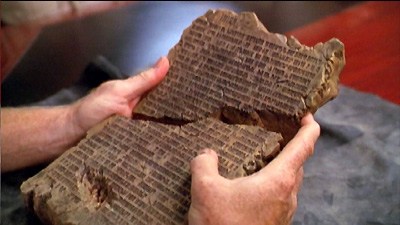
\includegraphics[width=0.5\textwidth]{ancienttablet.jpg}
\end{figure}

\section{Introduction}
Historically, a tablet is a chunk of stone of clay that ancient cultures used to write on. They were large, clunky, and hard to carry. In addition they easily cracked and broken. Modern day electronic tablets obviously are not nearly as chunky and heavy but many of the characteristics of ancient tablets still hold true to modern day ones. Both ancient and modern tablets are fixed in size and they are not the easiest to carry. And they crack and break very easily, especially when dropped. Yet for some reason, tablets these days are all the rage. Apple iPad, the Google Nexus, the Samsung Galaxy Tab, the Windows Surface are all very popular buys as they aim to find the middle ground between a mobile phone and a laptop. But tablets these days just don't enough. Their design has failed to provide a successful model to find that portable device that is the middle ground between a computer and a mobile phone. The tablet's time is done. Ancient tablets were eventually replaced with the far more efficient paper. Paper took on many various forms but one of the most efficient was the scroll. And that is were we come in. It's time to replace the modern day computing tablet with the next step in it's evolution. It is time for the modern computer scroll. The following is our proposed design for a computing scroll, the Scrollet.

\section{The System of Use}
\label{sec:system}
The Scrollet is designed to be that middle ground that tablets just never could be. Compressible, efficient, flexible and multifaceted the Scrollet can be used for anything. It can stand upright on by itself, hang from a wall, or tilt at an angle with a kickstand. It can run any touch based operating system. It has stylus and bluetooth keyboard capability. In addition it has everything a tablet has such as front and rear-facing cameras, USB port, speakers, accelerometers and more. The innovation comes with the flexible screen rolls up into the sides of the scrolls.

\subsection{Potential Usability Issues}
There is no such thing as a perfect product and the Scrollet definitely has some usability issues. The biggest of these is how a user touch input would work on such a thin, flexible screen. If the user input is too hard the screen bend. Screen stability and integrity are a huge concern. Just because the screen is flexible does not mean it is unbreakable. The screen could very easily potentially rip or tear. Another usability issue is battery life. The Scrollet is a powerful device and it is uncertain how long it will last when portable. 

\section{Top Level Design}
\subsection{Hardware Overview}
The Scrollet, naturally, is designed like to work like a scroll. It has two "Grabbles" on the sides from which the screen rolls into. When the Scrollet is closed, all that is visible are the two Grabbles. There is a manual push switch that can be used to lock the Scrollet in closed position. Upon pulling the Grabbles apart, a thin, flexible screen comes out. Upon being fully pulled out, a switch will trip and the screen will lock in the out position. The switch is tripped by pulling the screen out to it's maximum length then releasing. To roll the screen back into the Grabbles, the switch is tripped again and will slowly pull the screen in itself with the user guiding it in.

\subsection{The Grabbles}
The Grabbles are where mostly everything occurs in the Scrollet. Their shape is parabolic but they are cylindrical in nature. Inside the Grabbles are the processor, memory, storage, graphics card, battery, speakers, accelerometers, compass, GPS, light sensors, WiFi antenna, Bluetooth chip. In addition, the inside of the grabbles will have some protective cushioning to better protect the screen and other critical components. On the exterior of the Grabbles are the HDMI input, Mini-Display input, headphone port, stylus slot, power button, camera, a USB 3.0 port for additional storage, a USB Micro port to be used for charging as well as syncing data to computers. On the backside of the Grabbles, there is an adjustable kickstand that can be used to prop up the Scrollet during use as well as two mounting holes that would allow for the Scrollet to be mounted on a wall.

\subsection{The Screen}
The screen is thin and flexible. It has the potential to be either transparent or non-transparent based on the user's choosing. It is touch sensitive and touch is the primary way users input information.

\subsection{Software Overview}
The root operating system of the Scrollet is a very simple touch-based operating system that offers very few options to the user. Its main purpose to serve as essentially a boot menu for the virtual guest systems that are run inside the root. That being said the root operating system has essentially 5 main functions.

\subsubsection{DisplayMode}
The first function is to enter DisplayMode. Display Mode allows for the Scrollet to be used as a external monitor for a computer. This can be done through the HDMI or MiniDisplay port as well as over Wi-Fi similarly to Apple AirPlay.

\subsubsection{MainMode}
MainMode is where most of the Scrollet's user usage will occur. Essentially MainMode is a virtual machine that allows for the user to run another operating system as a guest system on top of the root operating system. Users will obviously only be able to use guest operating systems that support touch interface. The 3 operating systems currently that would be considered able to be used on Scrollet are Windows 8.1, Android OS for tablets, and iOS for tablets. They would use virtual hard disks for storage.

\subsubsection{CameraMode}
CameraMode is a simple function that allows for users to access and use the camera without having to boot up into a virtual operating system.

\subsubsection{MusicPlayer}
The music player allows for the user to access and play their music library without having to boot into a virtual system to have their music at their fingertips.

\subsubsection{Settings}
The final function on the root operating system is Settings. Settings is, naturally, where all of the settings for the Scrollet can be accessed. Here users can modify the settings for any virtual operating system they are running and access other device settings.




\section{Usage Scenarios}
\subsection{As A External Monitor}
'

\subsection{As Computing Tablet-Style Device}

\section{Why Scrollet}

\subsection{Priorities}
\subsection{Mental Models, Design Concepts, Principles, Theories}

\section{Usability Metric Analysis}

\section{Conclusion}

\end{document}